\documentclass[12pt,a4paper]{article}
\usepackage[utf8]{vietnam}
\usepackage{amsmath,amssymb}
\usepackage{geometry}
\geometry{top=1.5cm,bottom=1.2cm,left=1.4cm,right=1.4cm,headheight=28pt,headsep=12pt,footskip=18pt}
\usepackage{tikz}
\usepackage{xcolor}
\usepackage{enumerate}
\usepackage{graphicx}
\usepackage[version=4]{mhchem}
\usepackage{fancyhdr}
\usepackage{ex_test}

\renewcommand{\baselinestretch}{0.96}
\setlength{\parskip}{0pt}

\definecolor{hfRed}{RGB}{211,47,47}
\definecolor{hfGreen}{RGB}{139,195,144}

\pagestyle{fancy}
\fancyhf{}
\fancyhead[L]{\small\itshape\color{hfRed} Tài liệu lưu hành nội bộ}
\fancyhead[R]{\small\itshape\color{hfRed} Thầy \textbf{TRẦN VĂN THẠNH} - 0777.470.803}
\renewcommand{\headrulewidth}{0.8pt}
\renewcommand{\headrule}{\hbox to\headwidth{\color{hfGreen}\leaders\hrule height \headrulewidth\hfill}}

\fancyfoot[L]{\small\itshape\color{hfRed} CS1: 6/15 Nguyễn Hoàng, P. Kim Long, TP Huế \quad|\quad CS2: 24 Đặng Thái Thân, TP Huế}
\fancyfoot[R]{\small\bfseries\color{hfRed} Trang \thepage}
\renewcommand{\footrulewidth}{0.8pt}
\renewcommand{\footrule}{\hbox to\headwidth{\color{hfGreen}\leaders\hrule height \footrulewidth\hfill}}

\fancypagestyle{firstpage}{
  \fancyhf{}
  \renewcommand{\headrulewidth}{0pt}
  \fancyfoot[L]{\small\itshape\color{hfRed} CS1: 6/15 Nguyễn Hoàng, P. Kim Long, TP Huế \quad|\quad CS2: 24 Đặng Thái Thân, TP Huế}
  \fancyfoot[R]{\small\bfseries\color{hfRed} Trang \thepage}
  \renewcommand{\footrulewidth}{0.8pt}
  \renewcommand{\footrule}{\hbox to\headwidth{\color{hfGreen}\leaders\hrule height \footrulewidth\hfill}}
}

\begin{document}
\thispagestyle{firstpage}

\noindent
\begin{minipage}[t]{0.44\textwidth}
	\centering\fontsize{10pt}{12pt}\selectfont
	\textbf{SỞ GIÁO DỤC VÀ ĐÀO TẠO THỪA THIÊN HUẾ}\\
	\textbf{ĐỀ CHÍNH THỨC}\\
	\textit{(Đề thi có 04 trang)}
\end{minipage}\hfill
\begin{minipage}[t]{0.54\textwidth}
	\centering\fontsize{10.5pt}{13pt}\selectfont
	\textbf{ĐỀ KIỂM TRA ĐỊNH KỲ CHƯƠNG 3 (ĐẠI CƯƠNG HÓA HỮU CƠ)}\\
	\textbf{MÔN: HOÁ HỌC - LỚP 11}\\
	\textit{Thời gian làm bài: 45 phút, không kể thời gian phát đề}
	
	\smallskip
	\fbox{\textbf{MÃ ĐỀ: 108}}
\end{minipage}

\smallskip
\begin{center}
	{\color{hfRed}\textbf{\large (BẢN GIÁO VIÊN -- CÓ LỜI GIẢI CHI TIẾT)}}
\end{center}

\smallskip
\noindent\hrulefill
\smallskip

\noindent\textbf{Họ, tên thí sinh:} \dotfill\ \textbf{Lớp:} \dotfill\ \textbf{Số báo danh:} \dotfill

\smallskip
\noindent\textit{(Cho biết nguyên tử khối: H = 1; C = 12; N = 14; O = 16; F = 19; Na = 23; Mg = 24; Al = 27; P = 31; S = 32; Cl = 35,5; K = 39; Ca = 40; Fe = 56; Cu = 64; Br = 80; Ag = 108).}
\smallskip

\noindent\textbf{\large PHẦN I. Câu trắc nghiệm nhiều phương án lựa chọn.}
\textit{Thí sinh trả lời từ câu 1 đến câu 18. Mỗi câu hỏi thí sinh chỉ chọn một phương án.}
\vspace{0.2cm}

\Opensolutionfile{ans}[ans-hoa11-de08gv]

\begin{ex}
\textbf{[KNTT - SBT]} Xét phản ứng quang hợp: $\ce{6CO2 + 6H2O -> C6H12O6 + 6O2}$. Chất nào trong phản ứng này thuộc loại hợp chất hữu cơ?
\choice
{$\ce{CO2}$}
{$\ce{H2O}$}
{\True $\ce{C6H12O6}$}
{$\ce{O2}$}

\loigiai{
$\ce{C6H12O6}$ (glucose) là hợp chất hữu cơ, các chất còn lại ($\ce{CO2, H2O, O2}$) là hợp chất vô cơ.
}
\end{ex}

\begin{ex}
\textbf{[KNTT - SBT]} Hydrocarbon là loại hợp chất hữu cơ mà thành phần phân tử có các nguyên tố nào sau đây?
\choice
{\True C và H}
{C, H và O}
{C, H và N}
{C, H, O và N}

\loigiai{
Hydrocarbon là loại hợp chất hữu cơ mà trong phân tử chỉ chứa hai nguyên tố carbon và hydrogen.
}
\end{ex}

\begin{ex}
\textbf{(SBT - CTST)} Phương pháp chưng cất dùng để tách các chất
\choice
{\True có nhiệt độ sôi khác nhau}
{có nhiệt độ nóng chảy khác nhau}
{có độ tan khác nhau}
{có khối lượng riêng khác nhau}

\loigiai{
Phương pháp chưng cất dựa trên sự khác nhau về nhiệt độ sôi của các chất lỏng trong hỗn hợp ở cùng áp suất.
}
\end{ex}

\begin{ex}
Chưng cất gồm bao nhiêu giai đoạn?
\choice
{1 giai đoạn: thay đổi điều kiện hoà tan}
{\True 2 giai đoạn: bay hơi và ngưng tụ}
{3 giai đoạn: đun nóng, bay hơi, ngưng tụ}
{4 giai đoạn: hoà tan, lọc nóng, để nguội, lọc chất kết tinh}

\loigiai{
Quá trình chưng cất gồm hai giai đoạn liên tiếp nhau: bay hơi (chuyển chất lỏng thành hơi khi sôi) và ngưng tụ (làm lạnh hơi chuyển lại thành chất lỏng).
}
\end{ex}

\begin{ex}
Glucose là hợp chất hữu cơ có nhiều trong các loại quả chín, đặc biệt là quả nho. Công thức phân tử của glucose là $\ce{C6H12O6}$. Công thức đơn giản nhất của glucose là
\choice
{$\ce{C_{1,5}H3O_{1,5}}$}
{\True $\ce{CH2O}$}
{$\ce{C3H4O3}$}
{$\ce{CHO2}$}

\loigiai{
Tỉ lệ số nguyên tử trong $\ce{C6H12O6}$ là $\text{N(C)} : \text{N(H)} : \text{N(O)} = 6 : 12 : 6 = 1 : 2 : 1 \Rightarrow$ Công thức đơn giản nhất là $\ce{CH2O}$.
}
\end{ex}

\begin{ex}
Phân tử khối của chất hữu cơ nào sau đây là 30?
\choice
{\True $\ce{HCHO}$}
{$\ce{C3H8}$}
{$\ce{C2H4}$}
{$\ce{C3H4}$}

\loigiai{
$M(\ce{HCHO}) = 1 + 12 + 1 + 16 = 30$. (Các chất khác: $M(\ce{C3H8}) = 44$, $M(\ce{C2H4}) = 28$, $M(\ce{C3H4}) = 40$).
}
\end{ex}

\begin{ex}
Hợp chất nào sau đây là đồng đẳng của acetic acid $\ce{CH3COOH}$?
\choice
{\True $\ce{HCOOH}$}
{$\ce{CH3COOCH3}$}
{$\ce{HOCH2COOH}$}
{$\ce{HOOC-COOH}$}

\loigiai{
Đồng đẳng của acetic acid (carboxylic acid no, đơn chức, mạch hở $\ce{C_nH_{2n}O2}$) là formic acid (methanoic acid) $\ce{HCOOH}$.
}
\end{ex}

\begin{ex}
\textbf{[KNTT - SBT]} Những hợp chất hữu cơ khác nhau nhưng có cùng công thức phân tử được gọi là các chất
\choice
{\True đồng phân của nhau}
{đồng đẳng của nhau}
{đồng vị của nhau}
{đồng khối của nhau}

\loigiai{
Các chất khác nhau nhưng có cùng công thức phân tử được gọi là các đồng phân của nhau.
}
\end{ex}

\begin{ex}
\textbf{[KNTT - SBT]} Biết rằng hydrocarbon no chỉ chứa liên kết đơn, hydrocarbon không no có chứa liên kết bội và hydrocarbon thơm có chứa vòng benzene. Xét các chất sau:
\begin{center}
	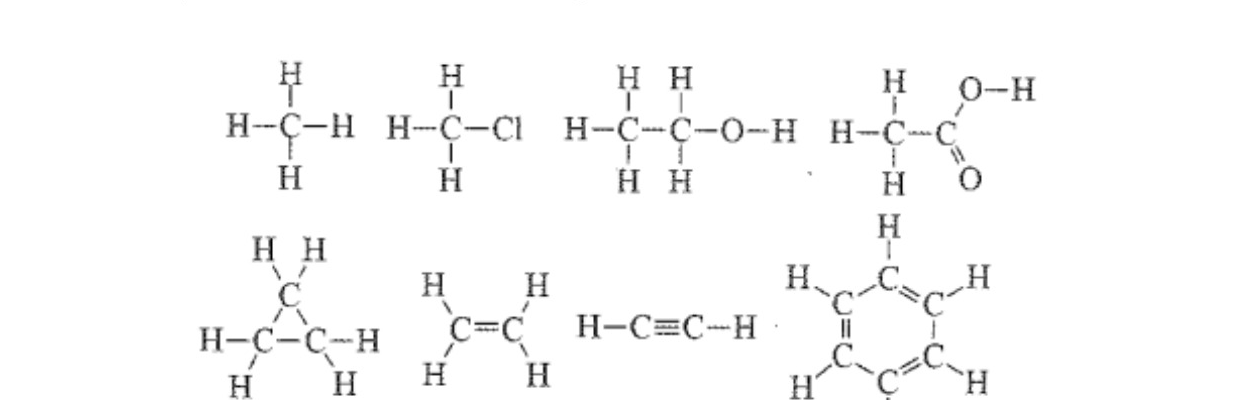
\includegraphics[width=13cm]{images_crop_hoa11_de08/cau9_p1_cau_truc_8chat.png}
\end{center}
Nhận định nào sau đây \textbf{không} đúng?
\choice
{số hydrocarbon bằng 5}
{số dẫn xuất hydrocarbon bằng 3}
{số hydrocarbon no bằng 2}
{\True số hydrocarbon không no bằng 3}

\loigiai{
Phân tích 8 chất trên:\\
- Dẫn xuất hydrocarbon gồm 3 chất: $\ce{CH3Cl}$, $\ce{CH3CH2OH}$, $\ce{CH3COOH} \Rightarrow$ B đúng.\\
- Hydrocarbon gồm 5 chất: $\ce{CH4}$, cyclopropane $\ce{C3H6}$, $\ce{C2H4}$, $\ce{C2H2}$, benzene $\ce{C6H6} \Rightarrow$ A đúng.\\
- Hydrocarbon no gồm 2 chất: $\ce{CH4}$ và cyclopropane $\Rightarrow$ C đúng.\\
- Hydrocarbon không no chỉ có 2 chất: ethylene $\ce{C2H4}$ và acetylene $\ce{C2H2}$; còn benzene $\ce{C6H6}$ là hydrocarbon thơm $\Rightarrow$ D sai ("số hydrocarbon không no bằng 3" là sai).
}
\end{ex}

\begin{ex}
\textbf{[KNTT - SBT]} Nhận định nào sau đây \textbf{không} đúng?
\choice
{$\ce{CH4, CH2=CH2}$ và $\ce{CH#CH}$ là những hydrocarbon}
{$\ce{CH3OH}$ và $\ce{HOCH2-CH2OH}$ là những alcohol}
{$\ce{CH3COOH}$ và $\ce{CH2(COOH)2}$ là những carboxylic acid}
{\True $\ce{CH3CH=O}$ và $\ce{CH3COCH3}$ là những aldehyde}

\loigiai{
$\ce{CH3COCH3}$ (acetone) là hợp chất ketone (chứa nhóm carbonyl liên kết trực tiếp với hai gốc hydrocarbon), không phải aldehyde. Do đó nhận định D không đúng.
}
\end{ex}

\begin{ex}
\textbf{[KNTT – SBT]} Trong quá trình chưng cất dầu thô, người ta thu được nhiều phân đoạn dầu mỏ, trong đó có xăng (thành phần chính là hỗn hợp các hydrocarbon có số nguyên tử C từ 4 đến 12, nhiệt độ sôi khoảng từ $40^\circ\text{C}$ đến $200^\circ\text{C}$) và dầu hoả (thành phần chính là hỗn hợp các hydrocarbon có số nguyên tử C từ 12 đến 16, nhiệt độ sôi khoảng từ $200^\circ\text{C}$ đến $250^\circ\text{C}$). Sản phẩm thu được ở $150^\circ\text{C}$ đến $200^\circ\text{C}$ là
\choice
{xăng}
{dầu hoả}
{\True xăng và dầu hoả}
{dầu hoả và xăng}

\loigiai{
Ở khoảng $150^\circ\text{C}$ đến $200^\circ\text{C}$, phân đoạn chưng cất có sự gối đầu giữa các hydrocarbon có khối lượng phân tử lớn của xăng và các hydrocarbon phân tử nhỏ của dầu hoả, do đó sản phẩm thu được gồm cả xăng và dầu hoả.
}
\end{ex}

\begin{ex}
\textbf{[KNTT – SBT]} Thêm benzene vào ống nghiệm đựng dung dịch nước bromine. Sau một thời gian quan sát thấy màu đỏ nâu của bromine
\choice
{chủ yếu trong lớp nước}
{\True chủ yếu trong lớp benzene}
{phân bố đồng đều ở hai lớp}
{bị mất màu hoàn toàn}

\loigiai{
Bromine tan trong dung môi không phân cực (benzene) tốt hơn rất nhiều so với trong dung môi phân cực (nước). Do đó bromine được chiết vào lớp benzene ở phía trên làm lớp benzene có màu đỏ nâu đậm.
}
\end{ex}

\begin{ex}
\textbf{(SBT - CĐ)} Sau khi biết công thức thực nghiệm, có thể xác định công thức phân tử của hợp chất hữu cơ dựa trên đặc điểm nào sau đây?
\choice
{\True Phân tử khối của chất}
{Thành phần phần trăm về khối lượng của các nguyên tố có trong phân tử chất}
{Khối lượng các sản phẩm thu được khi đốt cháy hoàn toàn một lượng chất xác định}
{Các hấp thụ đặc trưng trên phổ IR của chất}

\loigiai{
Công thức phân tử $= (\text{CTTN})_n$. Khi biết phân tử khối $M$, ta xác định được hệ số $n = M / M_{\text{CTTN}}$, từ đó suy ra công thức phân tử.
}
\end{ex}

\begin{ex}
\textbf{(SBT - KNTT)} Hình sau đây là phổ khối lượng của phân tử acetic acid:
\begin{center}
	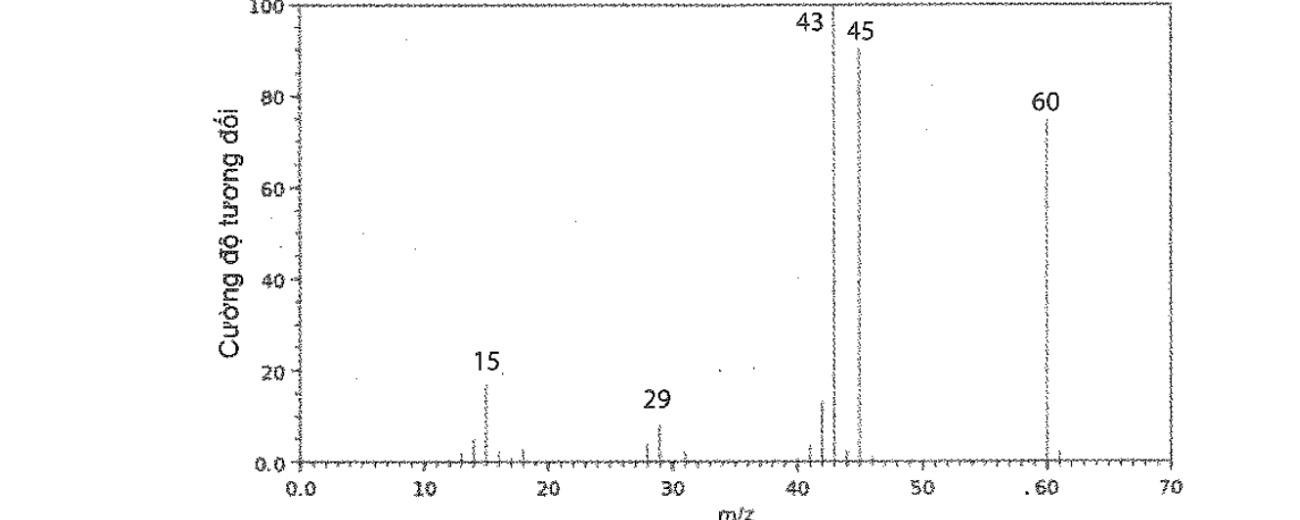
\includegraphics[width=9cm]{images_crop_hoa11_de08/cau14_p1_ms_acetic_acid.png}
\end{center}
Phân tử khối của acetic acid bằng
\choice
{43}
{45}
{\True 60}
{29}

\loigiai{
Trên phổ MS, peak ion phân tử $[\ce{M+}]$ có giá trị $m/z$ lớn nhất là 60. Do đó phân tử khối của acetic acid bằng 60.
}
\end{ex}

\begin{ex}
Cho các cặp chất:
\begin{enumerate}[(1)]
	\item $\ce{CH3CH2OH}$ và $\ce{CH3OCH3}$
	\item $\ce{CH3CH2Br}$ và $\ce{BrCH2CH3}$
	\item $\ce{CH2=CH-CH2OH}$ và $\ce{CH3CH2CHO}$
	\item $\ce{(CH3)2NH}$ và $\ce{CH3CH2NH2}$
\end{enumerate}
Có bao nhiêu cặp là đồng phân cấu tạo?
\choice
{1}
{2}
{\True 3}
{4}

\loigiai{
- Cặp (1): Cùng $\ce{C2H6O}$ (alcohol và ether) $\Rightarrow$ đồng phân cấu tạo.\\
- Cặp (2): $\ce{CH3CH2Br}$ và $\ce{BrCH2CH3}$ là cùng một chất bromoethane $\Rightarrow$ không phải đồng phân.\\
- Cặp (3): Cùng $\ce{C3H6O}$ (alcohol không no và aldehyde) $\Rightarrow$ đồng phân cấu tạo.\\
- Cặp (4): Cùng $\ce{C2H7N}$ (amine bậc 2 và amine bậc 1) $\Rightarrow$ đồng phân cấu tạo.\\
Vậy có 3 cặp là đồng phân cấu tạo (1, 3, 4).
}
\end{ex}

\begin{ex}
Cho chất acetylene ($\ce{C2H2}$) và benzene ($\ce{C6H6}$), hãy chọn nhận xét \textbf{đúng} trong các nhận xét sau đây:
\choice
{Hai chất đó giống nhau về công thức phân tử và khác nhau về công thức đơn giản nhất}
{\True Hai chất đó khác nhau về công thức phân tử và giống nhau về công thức đơn giản nhất}
{Hai chất đó khác nhau về công thức phân tử và khác nhau về công thức đơn giản nhất}
{Hai chất đó có cùng công thức phân tử và cùng công thức đơn giản nhất}

\loigiai{
$\ce{C2H2}$ và $\ce{C6H6}$ có công thức phân tử khác nhau, nhưng đều có tỉ lệ nguyên tử $\text{C} : \text{H} = 1 : 1$ nên có cùng công thức đơn giản nhất là $\ce{CH}$.
}
\end{ex}

\begin{ex}
Methadone là một loại thuốc dùng trong cai nghiện ma túy, nó thực chất cũng là một loại chất gây nghiện nhưng ``nhẹ'' hơn các loại ma túy thông thường và dễ kiểm soát hơn. Công thức cấu tạo của methadone như hình dưới:
\begin{center}
	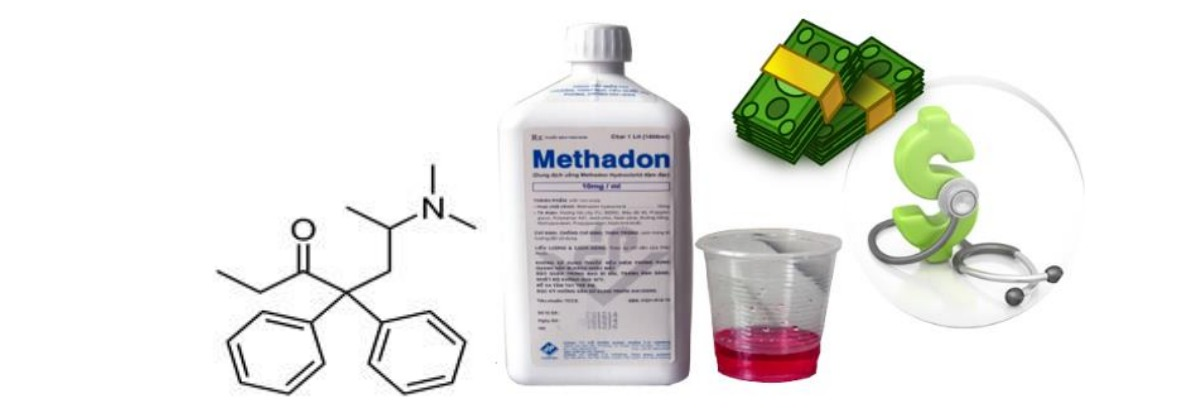
\includegraphics[width=10.5cm]{images_crop_hoa11_de08/cau17_p1_methadone.png}
\end{center}
Công thức phân tử của methadone là
\choice
{$\ce{C17H27NO}$}
{$\ce{C17H22NO}$}
{$\ce{C21H29NO}$}
{\True $\ce{C21H27NO}$}

\loigiai{
Đếm số nguyên tử từ cấu trúc:\\
- Số nguyên tử C: 2 vòng benzene (12 C) + C bậc 4 (1 C) + nhóm $-\ce{CO-CH2CH3}$ (3 C) + mạch $-\ce{CH2-CH(CH3)-N(CH3)2}$ (5 C) $\Rightarrow$ Tổng cộng có 21 carbon.\\
- Độ bất bão hòa $k = 2 \times 4$ (2 vòng benzene) $+ 1\ (\ce{C=O}) = 9 \Rightarrow$ Số nguyên tử $\text{H} = 2 \times 21 + 2 + 1 - 2 \times 9 = 27$.\\
- Phân tử chứa 1 nguyên tử N và 1 nguyên tử O $\Rightarrow$ CTPT là $\ce{C21H27NO}$.
}
\end{ex}

\begin{ex}
Cho các phát biểu về đặc điểm chung của các phân tử hợp chất hữu cơ:
\begin{enumerate}[(a)]
	\item Thành phần nguyên tố chủ yếu là C và H.
	\item Có thể chứa nguyên tố khác như Cl, N, P, O.
	\item Liên kết hóa học chủ yếu là liên kết cộng hoá trị.
	\item Liên kết hoá học chủ yếu là liên kết ion.
	\item Dễ bay hơi, khó cháy.
	\item Phản ứng hoá học xảy ra nhanh.
\end{enumerate}
Các phát biểu đúng là
\choice
{4}
{\True 3}
{2}
{1}

\loigiai{
Các phát biểu đúng gồm: (a), (b), (c) $\Rightarrow$ Có 3 phát biểu đúng.\\
- (d) sai vì liên kết chủ yếu là liên kết cộng hóa trị.\\
- (e) sai vì hợp chất hữu cơ thường kém bền nhiệt và dễ cháy.\\
- (f) sai vì phản ứng của hợp chất hữu cơ thường xảy ra chậm và theo nhiều hướng.
}
\end{ex}

\Closesolutionfile{ans}
\newpage

\noindent\textbf{\large PHẦN II. Câu trắc nghiệm đúng sai.}
\textit{Thí sinh trả lời từ câu 1 đến câu 4. Trong mỗi ý a), b), c), d) ở mỗi câu, thí sinh chọn đúng hoặc sai.}
\vspace{0.2cm}

\begin{ex}
Đặc điểm chung của các phân tử hợp chất hữu cơ:
\choiceTF
{\True a) Thành phần nguyên tố chủ yếu là C và H}
{\True b) Liên kết hóa học chủ yếu là liên kết cộng hoá trị}
{c) Liên kết hoá học chủ yếu là liên kết ion}
{d) Dễ bay hơi, khó cháy}

\loigiai{
\begin{itemize}
	\item a) \textbf{Đúng}: Thành phần phân tử hợp chất hữu cơ bắt buộc có carbon, thường có hydrogen.
	\item b) \textbf{Đúng}: Liên kết hóa học chủ yếu trong hợp chất hữu cơ là liên kết cộng hóa trị.
	\item c) \textbf{Sai}: Hợp chất hữu cơ chủ yếu chứa liên kết cộng hóa trị, liên kết ion chỉ xuất hiện trong muối hữu cơ.
	\item d) \textbf{Sai}: Các hợp chất hữu cơ thường kém bền nhiệt và dễ cháy.
\end{itemize}
}
\end{ex}

\begin{ex}
Một mẫu hoa hoè được xác định có hàm lượng rutin là 26\%. Người ta đun sôi hoa hoè với nước ($100^\circ\text{C}$) để chiết lấy rutin. Biết độ tan của rutin là 5,2 gam trong 1 lít nước ở $100^\circ\text{C}$ và là 0,125 gam trong 1 lít nước ở $25^\circ\text{C}$.
\choiceTF
{a) Trong 100 gam hoa hòe có 30 gam rutin}
{\True b) Cần dùng tối thiểu 5 lít nước để chiết được lượng rutin có trong 100 gam hoa hoè}
{c) Giả thiết rằng toàn bộ lượng rutin trong hoa hoè đã tan vào nước khi chiết. Làm nguội dung dịch chiết 100 gam hoa hoè ở trên từ $100^\circ\text{C}$ xuống $25^\circ\text{C}$ thì thu được 28,0 gam rutin kết tinh}
{\True d) Khi tăng lượng nước, lượng rutin hoà tan trong dung dịch ở $25^\circ\text{C}$ tăng lên nên lượng rutin kết tinh bị giảm đi}

\loigiai{
\begin{itemize}
	\item a) \textbf{Sai}: Khối lượng rutin có trong 100 g hoa hoè là: $100 \times 26\% = 26\text{ gam}$ (không phải 30 gam).
	\item b) \textbf{Đúng}: Thể tích nước sôi ở $100^\circ\text{C}$ tối thiểu cần dùng là: $V = 26 / 5,2 = 5\text{ (lít)}$.
	\item c) \textbf{Sai}: Lượng rutin còn tan lại trong 5 lít nước ở $25^\circ\text{C}$ là: $5 \times 0,125 = 0,625\text{ g} \Rightarrow$ Lượng rutin kết tinh tách ra là: $26 - 0,625 = 25,375\text{ gam}$ (khác 28,0 gam).
	\item d) \textbf{Đúng}: Vì $m_{\text{tan}(25^\circ\text{C})} = V \times 0,125\text{ g}$, nếu tăng $V$ thì lượng rutin tan lại tăng, dẫn tới lượng rutin kết tinh $m_{\text{kt}} = m_{\text{ban đầu}} - m_{\text{tan}}$ bị giảm.
\end{itemize}
}
\end{ex}

\begin{ex}
Khi nghiên cứu thành phần hoá học của tinh dầu quế, người ta thu được nhiều hợp chất hữu cơ trong đó có cinnamaldehyde và o–methoxycinnamaldehyde với công thức cấu tạo:
\begin{center}
	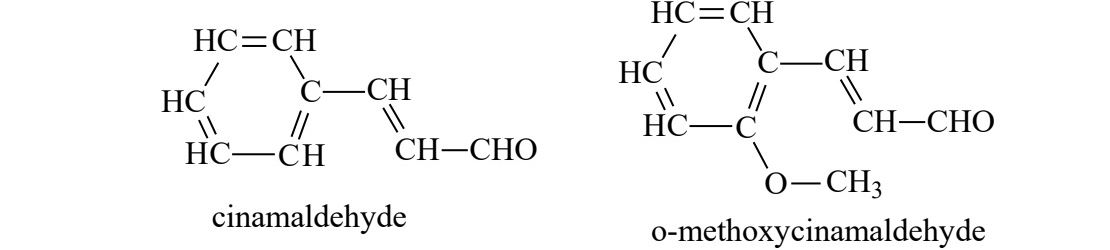
\includegraphics[width=11cm]{images_crop_hoa11_de08/cau3_p2_cinnamaldehyde.png}
\end{center}
Hãy chọn phát biểu Đúng hoặc Sai:
\choiceTF
{\True a) Công thức phân tử cinnamaldehyde: $\ce{C9H8O}$}
{\True b) Công thức đơn giản nhất cinnamaldehyde: $\ce{C9H8O}$}
{c) Công thức phân tử o–methoxycinnamaldehyde: $\ce{C5H5O}$}
{d) Công thức đơn giản nhất: $\ce{C10H10O2}$}

\loigiai{
\begin{itemize}
	\item a) \textbf{Đúng}: Cinnamaldehyde có gốc $\ce{C6H5-CH=CH-CHO}$ gồm 9 C, 8 H, 1 O $\Rightarrow$ CTPT là $\ce{C9H8O}$.
	\item b) \textbf{Đúng}: Tỉ lệ 9 : 8 : 1 không thể tối giản thêm, do đó CTĐGN trùng CTPT là $\ce{C9H8O}$.
	\item c) \textbf{Sai}: o-methoxycinnamaldehyde có công thức phân tử là $\ce{C10H10O2}$ ($\ce{C5H5O}$ là công thức đơn giản nhất).
	\item d) \textbf{Sai}: Tỉ lệ số nguyên tử là $10 : 10 : 2 = 5 : 5 : 1 \Rightarrow$ Công thức đơn giản nhất là $\ce{C5H5O}$, không phải $\ce{C10H10O2}$.
\end{itemize}
}
\end{ex}

\begin{ex}
Vanilin là hợp chất thiên nhiên, được sử dụng rộng rãi với chức năng phụ gia bổ sung hương thơm trong các loại đồ ăn, đồ uống, bánh kẹo, nước hoa,... Vanilin có cấu tạo như sau:
\begin{center}
	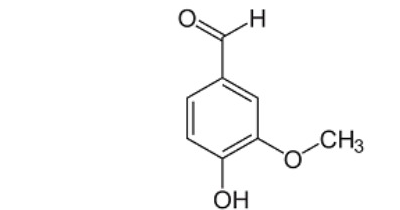
\includegraphics[width=4.5cm]{images_crop_hoa11_de08/cau4_p2_vanilin.png}
\end{center}
\choiceTF
{\True a) Phân tử vanilin có nhóm chức aldehyde}
{b) Phân tử vanilin có chứa nhóm chức alcohol}
{\True c) Vanilin có công thức phân tử $\ce{C8H8O3}$}
{\True d) Vanilin thuộc loại hợp chất hữu cơ tạp chức}

\loigiai{
\begin{itemize}
	\item a) \textbf{Đúng}: Phân tử vanilin có nhóm chức $-\ce{CHO}$ (aldehyde) gắn vào vòng thơm.
	\item b) \textbf{Sai}: Nhóm $-\ce{OH}$ gắn trực tiếp vào nguyên tử C của vòng thơm nên là nhóm chức phenol, không phải alcohol.
	\item c) \textbf{Đúng}: Đếm số nguyên tử: vòng $\ce{C6H3} + -\ce{CHO}\ (1\text{C}, 1\text{H}, 1\text{O}) + -\ce{OCH3}\ (1\text{C}, 3\text{H}, 1\text{O}) + -\ce{OH}\ (1\text{H}, 1\text{O}) \Rightarrow$ CTPT là $\ce{C8H8O3}$.
	\item d) \textbf{Đúng}: Vanilin chứa đồng thời các nhóm chức khác nhau: aldehyde ($-\ce{CHO}$), ether ($-\ce{OCH3}$), phenol ($-\ce{OH}$) nên là hợp chất hữu cơ tạp chức.
\end{itemize}
}
\end{ex}

\vspace{0.2cm}
\noindent\textbf{\large PHẦN III. Câu trắc nghiệm yêu cầu trả lời ngắn.}
\textit{Thí sinh trả lời từ câu 1 đến câu 6.}
\vspace{0.2cm}

\begin{ex}
Có bao nhiêu hydrocarbon trong số các chất dưới đây:
\[ \ce{CH4, NH3, C2H2, CCl4, C2H4, C6H6} \]

\loigiai{
\textbf{Đáp số: 4}\\
Các hydrocarbon (hợp chất chỉ tạo bởi C và H) gồm 4 chất: $\ce{CH4, C2H2, C2H4, C6H6}$. ($\ce{NH3}$ là chất vô cơ, $\ce{CCl4}$ là dẫn xuất halogen).
}
\end{ex}

\begin{ex}
Cây neem (cây thường xanh Ấn Độ) hay còn gọi là cây nim, sầu đâu (tên khoa học \textit{Azadirachta indica}) được người Ấn Độ dùng hơn 4000 năm nay để làm đẹp và chữa bệnh. Các chiết xuất từ lá neem có thể ức chế sự sao chép của virus Dengue, kháng virus nên có tác dụng điều trị bệnh sốt xuất huyết hiệu quả. Người ta hái một ít lá neem tươi, rửa sạch, cho vào nồi đun kĩ, lọc lấy nước để sử dụng. Hãy cho biết cách làm trên thuộc loại phương pháp tách và tinh chế nào (số thứ tự nào) trong các phương pháp sau:
\begin{center}
	1) Chưng cất; \quad 2) Chiết; \quad 3) Kết tinh; \quad 4) Sắc kí
\end{center}

\loigiai{
\textbf{Đáp số: 2}\\
Cách đun lá neem với nước sôi để hòa tan các dược chất từ mô thực vật vào nước rồi lọc lấy dịch chiết là phương pháp chiết lỏng -- rắn (phương pháp số 2).
}
\end{ex}

\begin{ex}
Phổ khối lượng của hợp chất hữu cơ X thu được như hình vẽ:
\begin{center}
	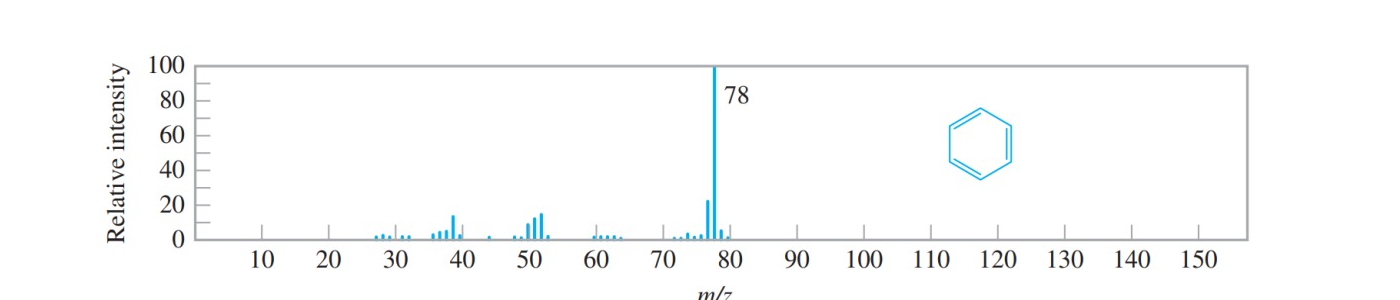
\includegraphics[width=10.5cm]{images_crop_hoa11_de08/cau3_p3_ms_benzene.png}
\end{center}
Phân tử khối của hợp chất hữu cơ X là?

\loigiai{
\textbf{Đáp số: 78}\\
Trên phổ MS, peak ion phân tử $[\ce{M+}]$ có giá trị $m/z$ lớn nhất bằng 78. Do đó phân tử khối của hợp chất X là 78 (chính là benzene $\ce{C6H6}$).
}
\end{ex}

\begin{ex}
Cho công thức sau:
\begin{center}
	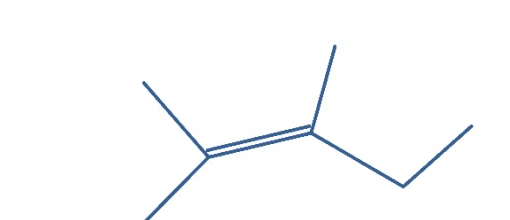
\includegraphics[width=5.5cm]{images_crop_hoa11_de08/cau4_p3_khung_alkene.png}
\end{center}
Hợp chất này có tổng số nguyên tử Carbon và Hydrogen là bao nhiêu?

\loigiai{
\textbf{Đáp số: 21}\\
Công thức khung phân tử biểu diễn một alkene mạch hở có 1 liên kết đôi $\ce{C=C}$:\\
- Mạch chính có 5 C, có 2 nhóm thế methyl ($-\ce{CH3}$) $\Rightarrow$ Tổng số nguyên tử C = 7.\\
- Hợp chất là alkene mạch hở có CTPT là $\ce{C7H14}$.\\
$\Rightarrow$ Tổng số nguyên tử C và H = $7 + 14 = 21$.
}
\end{ex}

\begin{ex}
Cho quy trình thực hiện thí nghiệm tinh chế benzoic acid:\\
Cân chính xác 1 gam benzoic acid thô cho vào bình định mức 250 mL. Cho từ từ nước sôi vào bình định mức và lắc đều cho đến khi benzoic acid tan hết. Tiến hành lọc nóng, để yên cho dung dịch nguội từ từ benzoic acid sẽ kết tinh. Lọc bằng máy hút chân không, thu được $m$ gam benzoic acid. Hiệu suất của quá trình kết tinh trên là 40\%. Giá trị của $m$ là bao nhiêu? (kết quả làm tròn đến hàng phần chục).

\loigiai{
\textbf{Đáp số: 0,4}\\
Khối lượng benzoic acid tinh khiết kết tinh thu được là:\\
$m = 1 \times 40\% = 0,4\text{ (g)}$.
}
\end{ex}

\begin{ex}
Camphor (có trong cây long não) là một chất rắn kết tinh màu trắng hay trong suốt giống như sáp với mùi thơm đặc trưng, thường dùng trong y học. Phần trăm khối lượng các nguyên tố trong camphor lần lượt là 78,94\% carbon, 10,53\% hydrogen và 10,53\% oxygen. Từ phổ khối lượng của camphor xác định được giá trị $m/z$ của peak $[\ce{M+}]$ bằng 152. Xác định số lượng nguyên tử của camphor.
\begin{center}
	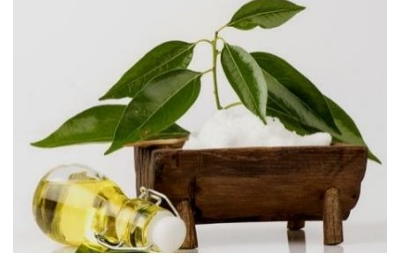
\includegraphics[width=4.5cm]{images_crop_hoa11_de08/cau6_p3_cay_long_nao.png}
	\qquad
	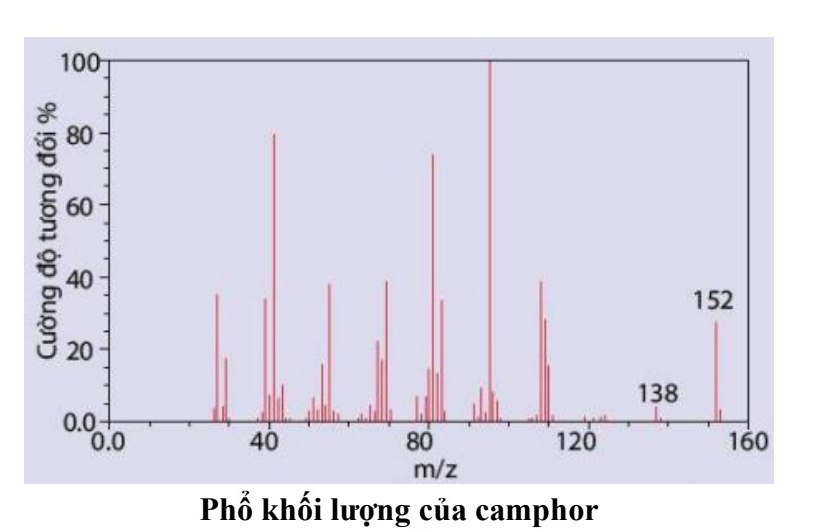
\includegraphics[width=9cm]{images_crop_hoa11_de08/cau6_p3_ms_camphor.png}
\end{center}

\loigiai{
\textbf{Đáp số: 27}\\
Đặt CTPT của camphor là $\ce{C_xH_yO_z}$ với $M = 152$:\\
- $x = \dfrac{152 \times 78,94\%}{12 \times 100\%} \approx 10$\\
- $y = \dfrac{152 \times 10,53\%}{1 \times 100\%} \approx 16$\\
- $z = \dfrac{152 \times 10,53\%}{16 \times 100\%} \approx 1$\\
$\Rightarrow$ CTPT của camphor là $\ce{C10H16O}$.\\
$\Rightarrow$ Tổng số lượng nguyên tử trong phân tử camphor là: $10 + 16 + 1 = 27$.
}
\end{ex}

\vspace{0.2cm}
\noindent\textbf{\large PHẦN IV. Tự luận.}
\textit{Thí sinh trình bày lời giải chi tiết cho các câu hỏi sau.}
\vspace{0.2cm}

\begin{ex}
\textbf{[CĐ-SGK]} Hãy xác định công thức đơn giản nhất của các hợp chất có công thức dưới đây:
\begin{enumerate}[a)]
	\item $\ce{C4H10}$ (butane)
	\item $\ce{HOCH2CH2OH}$ (ethane-1,2-diol)
	\item $\ce{C6H6}$ (benzene)
	\item $\ce{CHCl2COOH}$ (dichloroethanoic acid)
\end{enumerate}

\loigiai{
\textbf{Hướng dẫn giải:}\\
\begin{itemize}
	\item a) Butane: CTPT là $\ce{C4H10}$. Tỉ lệ $\text{C} : \text{H} = 4 : 10 = 2 : 5 \Rightarrow$ Công thức đơn giản nhất là $\ce{C2H5}$.
	\item b) Ethane-1,2-diol: CTPT là $\ce{C2H6O2}$. Tỉ lệ $\text{C} : \text{H} : \text{O} = 2 : 6 : 2 = 1 : 3 : 1 \Rightarrow$ Công thức đơn giản nhất là $\ce{CH3O}$.
	\item c) Benzene: CTPT là $\ce{C6H6}$. Tỉ lệ $\text{C} : \text{H} = 6 : 6 = 1 : 1 \Rightarrow$ Công thức đơn giản nhất là $\ce{CH}$.
	\item d) Dichloroethanoic acid: CTPT là $\ce{C2H2Cl2O2}$. Tỉ lệ $\text{C} : \text{H} : \text{Cl} : \text{O} = 2 : 2 : 2 : 2 = 1 : 1 : 1 : 1 \Rightarrow$ Công thức đơn giản nhất là $\ce{CHClO}$ (theo cách viết gom nhóm trong tài liệu gốc là $\ce{C2H2O2Cl}$).
\end{itemize}
}
\end{ex}

\begin{ex}
\textbf{[SBT - CTST]} Acetic acid được sử dụng rộng rãi trên thế giới trong nhiều ngành công nghiệp khác nhau như tạo ra polymer ứng dụng trong sơn, chất kết dính, là dung môi hoà tan các chất hoá học, sản xuất và bảo quản thực phẩm đặc biệt dùng để sản xuất giấm.
\begin{enumerate}[a)]
	\item Lập công thức phân tử của acetic acid, biết kết quả phân tích nguyên tố của acetic acid có 40\% C; 53,33\% O về khối lượng; còn lại là H. Phân tử khối của acetic acid được xác định trên phổ khối lượng tương ứng với peak có giá trị $m/z$ lớn nhất.
	\begin{center}
		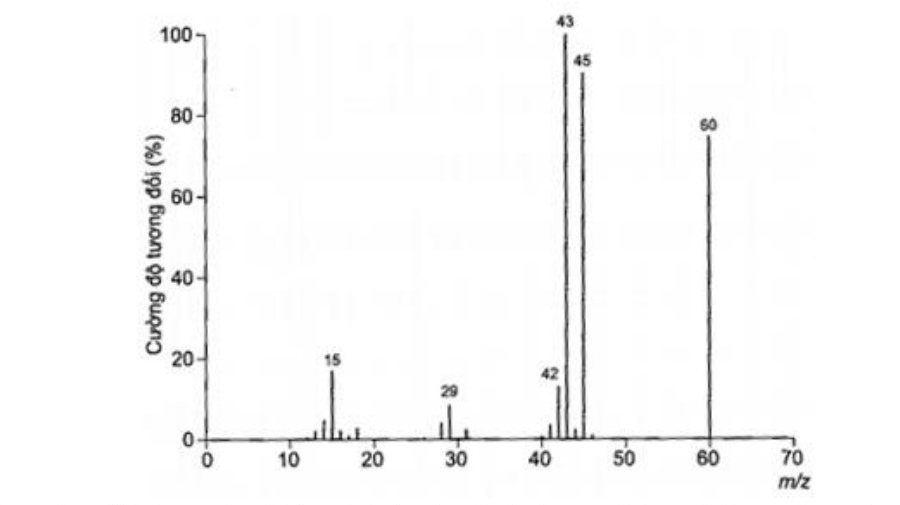
\includegraphics[width=9cm]{images_crop_hoa11_de08/cau2_p4_ms_acetic_acid.png}
	\end{center}
	\item Dựa vào phổ IR bên, hãy cho biết có thể xác định được nhóm chức carboxyl có trong acetic acid từ peak nào.
	\begin{center}
		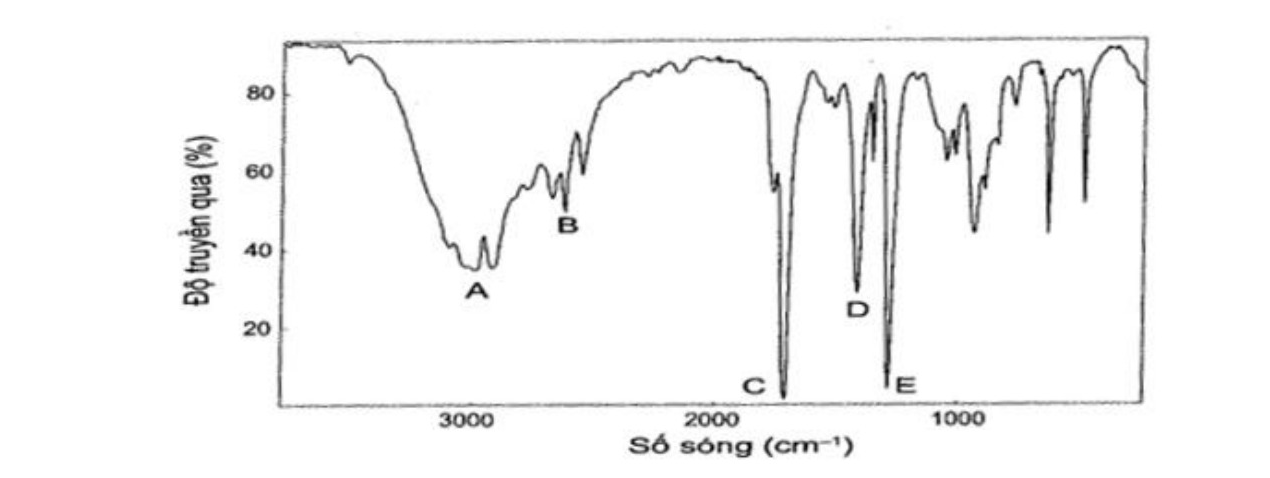
\includegraphics[width=11cm]{images_crop_hoa11_de08/cau2_p4_ir_acetic_acid.png}
	\end{center}
\end{enumerate}

\loigiai{
\textbf{Hướng dẫn giải:}\\
\begin{itemize}
	\item a) Tính thành phần \%H:
	\[ \%m_{\text{H}} = 100\% - 40\% - 53,33\% = 6,67\%. \]
	Từ phổ khối lượng (MS), peak ion phân tử $[\ce{M+}]$ có $m/z$ lớn nhất bằng 60 $\Rightarrow M_{\text{acetic acid}} = 60$.\\
	Đặt công thức phân tử của acetic acid là $\ce{C_xH_yO_z}$:\\
	$\bullet\ x = \dfrac{60 \times 40\%}{12 \times 100\%} = 2$\\
	$\bullet\ y = \dfrac{60 \times 6,67\%}{1 \times 100\%} \approx 4$\\
	$\bullet\ z = \dfrac{60 \times 53,33\%}{16 \times 100\%} \approx 2$\\
	$\Rightarrow$ Công thức phân tử của acetic acid là $\ce{C2H4O2}$.
	
	\item b) Dựa vào phổ hồng ngoại (IR):\\
	- Peak A (trong khoảng $3300 - 3000\text{ cm}^{-1}$, tù và rộng) đặc trưng cho dao động hóa trị của nhóm $\ce{O-H}$ liên kết trong nhóm carboxyl.\\
	- Peak C (ở khoảng $1700\text{ cm}^{-1}$, cường độ mạnh) đặc trưng cho dao động hóa trị của liên kết $\ce{C=O}$.\\
	Sự hiện diện đồng thời của peak A và peak C giúp xác định sự có mặt của nhóm chức carboxyl ($-\ce{COOH}$) trong phân tử acetic acid.
\end{itemize}
}
\end{ex}

\newpage
\begin{center}
	{\color{hfRed}\textbf{\Large BẢNG ĐÁP ÁN VÀ LỜI GIẢI CHI TIẾT}}
\end{center}
\vspace{0.3cm}

\noindent
\textbf{1. PHẦN I (Mỗi câu trả lời đúng thí sinh được 0,25 điểm):}
\begin{center}
\begin{tabular}{|c|c|c|c|c|c|c|c|c|}
\hline
\textbf{1. C} & \textbf{2. A} & \textbf{3. A} & \textbf{4. B} & \textbf{5. B} & \textbf{6. A} & \textbf{7. A} & \textbf{8. A} & \textbf{9. D} \\ \hline
\textbf{10. D} & \textbf{11. C} & \textbf{12. B} & \textbf{13. A} & \textbf{14. C} & \textbf{15. C} & \textbf{16. B} & \textbf{17. D} & \textbf{18. B} \\ \hline
\end{tabular}
\end{center}

\noindent
\textbf{2. PHẦN II (Trắc nghiệm đúng sai):}
\begin{itemize}
	\item \textbf{Câu 1:} a) Đúng \quad|\quad b) Đúng \quad|\quad c) Sai \quad|\quad d) Sai
	\item \textbf{Câu 2:} a) Sai \quad|\quad b) Đúng \quad|\quad c) Sai \quad|\quad d) Đúng
	\item \textbf{Câu 3:} a) Đúng \quad|\quad b) Đúng \quad|\quad c) Sai \quad|\quad d) Sai
	\item \textbf{Câu 4:} a) Đúng \quad|\quad b) Sai \quad|\quad c) Đúng \quad|\quad d) Đúng
\end{itemize}

\noindent
\textbf{3. PHẦN III (Trả lời ngắn):}
\begin{center}
\begin{tabular}{|c|c|c|c|c|c|}
\hline
\textbf{Câu 1} & \textbf{Câu 2} & \textbf{Câu 3} & \textbf{Câu 4} & \textbf{Câu 5} & \textbf{Câu 6} \\ \hline
4 & 2 & 78 & 21 & 0,4 & 27 \\ \hline
\end{tabular}
\end{center}

\begin{center}
\textbf{--------- HẾT ---------}
\end{center}

\end{document}
